% $Id: usbs.tex 9835 2022-02-13 02:57:36Z mskala $

%
% Low-level USB driver
% Copyright (C) 2022  Matthew Skala
%
% This program is free software: you can redistribute it and/or modify
% it under the terms of the GNU General Public License as published by
% the Free Software Foundation, version 3.
%
% This program is distributed in the hope that it will be useful,
% but WITHOUT ANY WARRANTY; without even the implied warranty of
% MERCHANTABILITY or FITNESS FOR A PARTICULAR PURPOSE.  See the
% GNU General Public License for more details.
%
% You should have received a copy of the GNU General Public License
% along with this program.  If not, see <http://www.gnu.org/licenses/>.
%
% Matthew Skala
% https://northcoastsynthesis.com/
% mskala@northcoastsynthesis.com
%

\chapter{Low-level USB driver (usb.s)}

The low-level USB driver in usb.s is responsible for all direct
communication with the PIC24's USB hardware; the per-device drivers operate
at a more abstract level, calling APIs provided by usb.s.  This module is
also responsible for overall management of the USB session.  It detects when
a device has been attached; handles reset, speed detection, and enumeration;
and after retrieving descriptors from the device, finds the appropriate
per-device driver to run.

In general, the Gracious Host low-level USB driver is designed to be the
smallest and simplest it can be while still basically working.  Many
features not relevant to the Gracious Host, such as hubs and isochronous
transfers, are not supported; and error checking is minimal.  This is not a
complete implementation of USB standards.

\section{Data structures}

The first section of the source file defines data structures used by the
low-level driver.  The BDT has a difficult alignment requirement, and most of
this module's data is statically allocated immediately after the BDT so that
it and the BDT can all be cleared with a two-instruction \insn{repeat} loop. 
Just a little bit of data specific to the device configuration process is
declared in the common area, because after configuration, the per-device
driver will own the common area.

\subsection{Buffer Descriptor Table (BDT)}

The USB hardware has a full complement of special function registers in the
SFR range at addresses 0x0480--0x04A8.  But it also uses a data structure in
general-purpose RAM to communicate with the driver.  This data structure has
a variable layout depending on whether the PIC24 is operating as host or
device, and also depending on various configuration options.  The RAM-based
data structure basically consists of an array called the Buffer Descriptor
Table (BDT) of two-word (32-bit) records, each of which may optionally point
at a buffer elsewhere in RAM.  The BDT itself must start aligned on a
512-byte (0x0200) boundary.  The buffers it points to apparently do not need
to be aligned at all -- they can start or end on odd bytes.

In full generality, each of the 16 endpoints has either two or four BDT
entries: one each for transmit and receive when \emph{ping-pong mode} is
disabled, doubled if ping-pong mode is enabled.  Then ping-pong mode can be
separately enabled or disabled for endpoint~0, and for all endpoints
\emph{other} than endpoint 0.  All in all, this makes for four different BDT
layouts, totalling 128, 132, 248, or 256 bytes (plus whatever the buffers
elsewhere consume).  However, in host mode (as used on the Gracious Host),
only endpoint~0 is used at all; and in the Gracious Host ping-pong mode is
disabled.  So the Gracious Host BDT really only consumes eight bytes, for
transmit and receive on endpoint~0.  The hardware promises (and apparently
is sincere) that in host mode it will not touch the other bytes that would
be part of the BDT in device mode.

The description of the BDT entry format is in the PIC24 \emph{DS} and
\emph{FRM}.  Each entry is basically one word of ``status'' information, and
a one-word address of the associated buffer.  The high bit of the status
word is called UOWN and serves as a semaphore or lock.  The usual pattern is
that this bit stays cleared when the BDT entry is not in use.  The software
sets up the buffer, then the BDT entry, including setting the UOWN bit. 
Then it writes other setup information to the SFRs, ending with a write to
U1TOK which triggers the hardware to actually make the transfer.  The
software (likely during an ISR) looks at UOWN to see when the hardware has
completed the transfer and cleared the bit, at which point the software is
free to use and change the data from the BDT entry and the buffer.  The
software is not allowed to write to the BDT entry or the buffer, and should
not trust data read from these places, while UOWN is set.

Ping-pong mode elaborates the handshaking by having two BDT entries
for each endpoint and direction, so that the software can be setting up or
tearing down one while the other is in use by the hardware.  In principle,
that should improve throughput.  In practice, the added complexity seems
unnecessary for the Gracious Host, and even Microchip's C-language driver,
although capable of enabling ping-pong mode, does not seem to be capable of
\emph{actually using} it to improve throughput.  As far as I can tell, the
Microchip driver will always wait for the current packet transfer to
complete and return UOWN before it starts working on another packet, making
ping-pong mode superfluous.  Maybe it could still have some advantage in
improving throughput between a background driver and foreground client.

\subsection{Endpoint (EP)}

The Gracious Host USB driver makes use of a 14-byte structure called an
endpoint (EP) which refers to one of the endpoints on the attached device. 
The static variables in usb.s include one of these, for endpoint~0, which is
implicitly used by the API calls for control transfers.  Per-device drivers
are expected to define their own and pass the addresses into the relevant
API calls when making non-control transfers.

Here is the layout of the EP structure.  It should be 16-bit aligned,
anywhere in RAM.

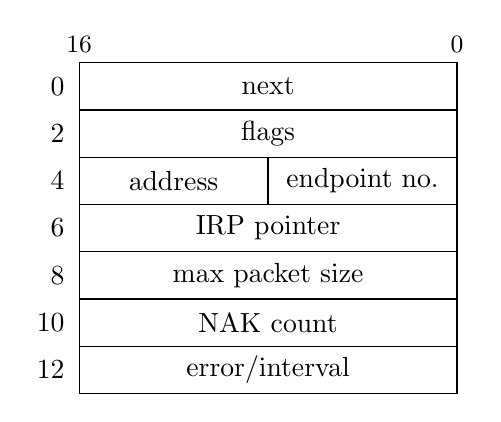
\begin{tikzpicture}[scale=0.3]
  \draw (0,0) rectangle (16,-14);
  \draw (0,-2) -- (16,-2);
  \draw (0,-4) -- (16,-4);
  \draw (8,-4) -- (8,-6);
  \draw (0,-6) -- (16,-6);
  \draw (0,-8) -- (16,-8);
  \draw (0,-10) -- (16,-10);
  \draw (0,-12) -- (16,-12);
  \draw (0,-14) -- (16,-14);
%
  \node[anchor=east] at (-0.2,-1) {0};
  \node[anchor=east] at (-0.2,-3) {2};
  \node[anchor=east] at (-0.2,-5) {4};
  \node[anchor=east] at (-0.2,-7) {6};
  \node[anchor=east] at (-0.2,-9) {8};
  \node[anchor=east] at (-0.2,-11) {10};
  \node[anchor=east] at (-0.2,-13) {12};
  \node[anchor=south] at (0,0) {\small 16};
  \node[anchor=south] at (16,0) {\small 0};
%
  \node at (8,-1) {next};
  \node at (8,-3) {flags};
  \node at (12,-5) {endpoint no.};
  \node at (4,-5) {address};
  \node at (8,-7) {IRP pointer};
  \node at (8,-9) {max packet size};
  \node at (8,-11) {NAK count};
  \node at (8,-13) {error/interval};
\end{tikzpicture}

Fields are as follows.

\begin{description}
  \item[next]  Pointer to the next endpoint.  These structures are meant to
    be arranged in a single-linked list using LL\_APPEND\_ATOMIC from
    utils.s.

  \item[flags]  Bit fields describing the type and status of the endpoint. 
    Constants for the Gracious Host-defined bit fields are in global.inc as
    symbols starting EPF\_ and EPFM\_.  The \emph{high byte} of this word
    (byte at offset 3) is a copy of the 8-bit \emph{bmAttributes} field from
    the USB endpoint descriptor returned by the device.

  \item[endpoint no.]  The byte at offset 4 is the 8-bit endpoint number on
    the device to which this structure connects.

  \item[address]  The byte at offset 5 is the 8-bit USB bus address of the
    device.  The Gracious Host always sets this to 1 during enumeration. 
    The reason for storing it in the EP structure at all is that bytes 4 and
    5 together form a 16-bit word in a format the hardware wants to see; and
    for the earliest control transfers that actually perform the
    enumeration, it may need to be zeroed.

  \item[IRP pointer]  Address in RAM of the IRP data structure (next
    subsection) that this endpoint is currently processing.

  \item[max packet size]  Maximum packet size the device supports for this
    endpoint, as it reported during configuration.  Set to guessed constants
    in early transfers, before the device has actually told the host what
    size it supports.

  \item[NAK count]  Count of the number of NAK packets, used for detecting
    the ``too many NAKs'' error condition on endpoints that do not allow
    infinite NAKs.

  \item[error/interval]  Normally, an error code.  Values are defined in
    global.inc, and some of them are set by the hardware.  A zero value,
    called ERR\_SUCCESS, corresponds to no error.  The occurrence of an error
    is also indicated by the IRPF\_ERROR bit in the IRP (not EP) flags
    field.  The EP error field is
    overloaded by the subroutines that configure INTR endpoints, to return
    the number of milliseconds at which the device requests to be polled. 
    The calling driver is expected to pick up this value from the field
    and store it somewhere safe before actually using the newly-configured
    endpoint, at which time the field will be used normally for error
    codes.
\end{description}

\subsection{I/O Request Packet (IRP)}

Another data structure used for communication between per-device drivers and
the low-level USB subsystem is called the I/O Request Packet (IRP).  Each
IRP describes a request for a transfer to or from the USB device.  The IRP
is separate from the EP so that a driver can maintain several of them for
different frequently-used kinds of transfers, and point the EP to different
IRPs to easily switch between them.

The IRP consists of an 8-byte header which points to a buffer.  For control
transfers in particular, the buffer is expected to immediately follow the
header, and to contain eight bytes at the start for the SETUP message
followed by space for the data payload if any.  For other types of transfers
(that is, interrupt and bulk; isochronous are not supported), the buffer may
be anywhere in RAM.

\pagebreak
Here is the IRP layout.

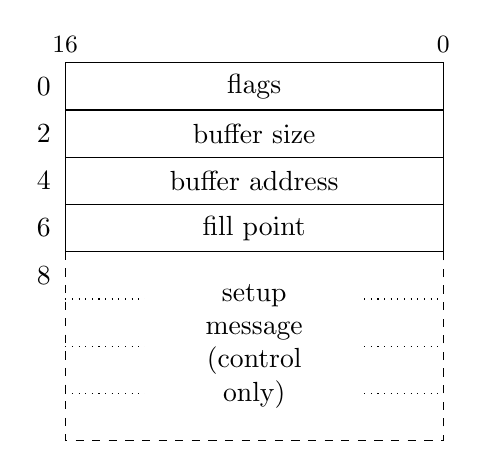
\begin{tikzpicture}[scale=0.3]
  \draw[dashed] (0,-8) rectangle (16,-16);
  \draw (0,0) rectangle (16,-8);
  \draw (0,-2) -- (16,-2);
  \draw (0,-4) -- (16,-4);
  \draw (0,-6) -- (16,-6);
  \draw[dotted] (0,-10) -- (16,-10);
  \draw[dotted] (0,-12) -- (16,-12);
  \draw[dotted] (0,-14) -- (16,-14);
%
  \node[anchor=east] at (-0.2,-1) {0};
  \node[anchor=east] at (-0.2,-3) {2};
  \node[anchor=east] at (-0.2,-5) {4};
  \node[anchor=east] at (-0.2,-7) {6};
  \node[anchor=east] at (-0.2,-9) {8};
  \node[anchor=south] at (0,0) {\small 16};
  \node[anchor=south] at (16,0) {\small 0};
%
  \node at (8,-1) {flags};
  \node at (8,-3) {buffer size};
  \node at (8,-5) {buffer address};
  \node at (8,-7) {fill point};
  \node[fill=white] at (8,-12)
    {\parbox{1in}{\centering setup\\message\\(control\\only)}};
\end{tikzpicture}

The fields are as follows.

\begin{description}
  \item[flags]  Bits describing the type and status of the request. 
    Note in particular that there is a UOWN flag for handshaking between the
    foreground and ISR in software, much like the handshaking between the
    software and hardware on BDT entries.  Constants for the bit fields are
    in global.inc as symbols starting IRPF\_ and IRPFM\_.

  \item[buffer size]  Size of the buffer.  This controls the transaction
    size.  The number here should include the setup message
    for control transactions (eight bytes), and any data payload.  Because
    the hardware sometimes overruns on DMA writes, it is advisable
    to actually allocate seven or eight bytes of padding after the
    buffer, which are not counted in the number of bytes stored here.

  \item[buffer address]  Address in RAM of the start of the buffer.  For
    \emph{control} transfers, this must point immediately after the IRP
    header structure (that is, at offset 8 from the start of the header). 
    For other transfers it may point anywhere.

  \item[fill point]  Offset into the buffer (that is, byte count, not
    address) of the next byte to transfer, or immediately after the last byte
    transferred.  Note that for control transfers, this will be 0 until the
    setup message is sent, then starts at 8 for the data bytes.

  \item[setup message]  The 8-byte setup message (for control transfers
    only) is formatted as described in the USB standard.
\end{description}

\section{Initialization and finalization}

The USB\_INIT subroutine sets up the USB hardware to listen for a device
attach.  It basically just loads appropriate values into the SFRs and turns
on the interrupts for device attach and 1\,ms timing.  Note that the USB
hardware potentially provides two different 1\,ms interrupts:  the ``On The
Go'' 1\,ms interrupt, which is available at all times and is the one turned
on here, and the ``SOF'' interrupt, which is only available when actually
sending SOFs or keep-alives to an attached USB device.  The SOF interrupt is
more accurately 1\,ms.  The Gracious Host switches between the two, using
the SOF interrupt for timing when possible but the 1\,ms interrupt at times
like these when SOF/keep-alive generation cannot be turned on.

USB\_DONE is even simpler:  it just turns off USB interrupts, clears a few
control registers, and clears the soft USB\_FLAGS variable.  If there should
still be a device attached at this point, the lack of SOFs or keep-alives
from the host will cause it to automatically shut down after a few
milliseconds.

Calling USB\_INIT when there is already a USB session in progress will break
the session off ungracefully, but should be safe from the driver's point of
view as long as the foreground keeps track of its own memory allocations and
other state.  It may be best not to do this while there is a \emph{transfer}
in progress, because the initialization includes the BDT and the hardware
could be attempting DMA at the time.  Calling USB\_DONE when there is no
session in progress, or when there has been no matching USB\_INIT call,
should be safe.

\section{Session handler}

The progress of the USB \emph{session}, from attach to detach, is handled by
the subroutine USB\_HANDLE\_SESSION.  Normally, the main loop in firmware.s
calls USB\_HANDLE\_SESSION when USB\_TEST\_ATTACHED returns NZ status; it is
expected, though not guaranteed in case of error, that the session handler
will remain in control until the USB device detach.  It ought to THROW in
case of an error that cannot be handled within the driver, but firmware.s is
also prepared to handle a simple return in an abnormal state, with the
device still attached.

The session handler is assembled into specially-named sections, not the
default .text, so that the customized linker script can insert code
fragments from other files to build up the executable TDL and TIL.  Devices
have device descriptors which say what kind of device they are, and code in
the TDL can match on those descriptors to call a driver for the entire
device.  Devices also have (potentially multiple) ``configurations,'' each
of which may contain (potentially multiple) ``interfaces,'' and each
\emph{interface} gets passed to the TIL for a possible match.  There is no
intermediate-level list for matching configurations; the matching is always
on the device or an interface, although an interface match will result in
the firmware selecting the associated configuration when setting up the
device.

\subsection{Sequence of events}

Several things have to happen in a specific sequence at the start of the
session to properly set up the USB device.  Here's a summary.  The structure
of the code follows the sequence quite closely.

\begin{itemize}
  \item Upon device attach, the session handler runs.  The caller has set
    both LEDs green.
  \item There is a 100\,ms pause for the power to stabilize.
  \item Check for low or full speed (USB\_TEST\_SPEED).  This point seems to
    be the only safe one for making this test; I had a lot of trouble trying
    to check the speed at other points in the sequence.  The left LED goes
    red if low speed.
  \item Send ``reset'' for 50\,ms.  Right LED goes red at the start of
    ``reset.''
  \item Start of SOF/keep-alive generation.  100\,ms pause for reset
    recovery.
  \item Prepare the static EP structure for endpoint~0, and a blank IRP
    structure in a \insn{lnk}/\insn{ulnk} stack frame.
  \item Reconfigure interrupts:  OTG 1\,ms off (from this point timing will
    use the SOF interrupt); SOF interrupts on; transfer complete, error, and
    detach on.  The ``detach'' interrupt flag is cleared first to ignore any
    stray detaches signalled prior to this point.  Sometimes contact bounce
    as the plug is inserted causes these.  If the device really detached
    during the roughly 250\,ms elapsed since attach was detected, and has
    remained detached, then that fact will be detected anyway as soon as the
    interrupt is enabled, because of the \emph{level-triggered} nature of
    the detach interrupt.
  \item ``Enumeration'':  do a zero-byte CTRL transfer telling the device
    that its address is~1 (unconditionally).  Call to do\_ctrl\_z\_transaction.
  \item Wait 5\,ms for the device to recover from enumeration.
  \item Do a CTRL read transfer for first~8 bytes of the device
    descriptor; call to do\_ctrl\_r\_transaction.
  \item Extract the actual size of the device descriptor from the 8-byte
    prefix just obtained.  It will almost certainly be~18 bytes, but doing
    this two-step process seems to be the expected procedure.  Do a CTRL
    read transfer for the entire device descriptor.  Copy the device
    descriptor (or, anyway, an 18-byte block from the buffer) to the local
    common-data variable saved\_dev\_desc to preserve it during TPL
    processing.  Update max packet size for EP~0 from the value in this
    descriptor.
  \item Check the device descriptor against the TDL (whole-device portion of
    the TPL).  The low-level driver sets up an exception frame and the TDL
    code is expected to THROW in case of a match.
  \item The linker inserts TDL fragments from all the drivers inside the
    exception frame.  The exception handler, if reached because of the THROW,
    jumps to the per-device driver which the TDL fragment selected by setting
    W4.  The exception handler also turns off the LEDs.
  \item Without a THROW, the session handler starts looping over
    configuration descriptors, using the count of configurations from the
    saved device descriptor.
  \item Request (EP max packet size) bytes of the current-index configuration descriptor with a
    CTRL read transaction.  Find the descriptor's actual size from the first
    few bytes; skip to the next one if it is too long for our buffer. 
    Buffer size is set to accommodate MAX\_DESCRIPTOR\_SIZE set in
    global.inc, currently 1023 bytes, plus appropriate headers and padding. 
    Descriptors we can reasonably use should never be longer than that.
    If descriptor is not too long for buffer, then request all of it with
    another CTRL read.  Save the start of this configuration descriptor (10
    bytes) in the common-data variable saved\_conf\_desc.
  \item The configuration descriptor is a pile of miscellaneous structures
    including its own header, one or more interface descriptor headers, and other
    things nested inside the interface descriptors.  Every item in the pile
    is tagged with a magic number saying what it is (though we do not
    necessarily understand all the types) and its length, and these
    fields are consistently laid out even if the rest of the item is opaque. 
    So there is a chunk of code to ``eat'' a descriptor from the bottom of
    the pile, moving everything after it down however many bytes to bring
    the next item to the start of the data buffer (right after the setup
    message).  This operation gets repeated until there is an interface
    descriptor header at the start of the buffer.
  \item Check the interface descriptor against the TIL.  As with the TDL,
    the session manager sets up an exception frame and the TDL entries from
    per-device drivers get inserted inside the frame by the linker.  If one
    THROWs, then the appropriate driver gets control, through the exception
    handler's \insn{goto}~W4 instruction.
  \item If no THROW, then the session handler loops around, removing items
    from the buffer until there is an interface descriptor at the start.  It
    knows how many interface descriptors are meant to exist in total, from a
    count in the saved configuration descriptor.
  \item If it gets through all the interface descriptors without a match, it
    loops to the next configuration descriptor.
  \item If still no match after the loop over all configurations, the
    session handler sets up an error display with the LED blinker driver,
    and waits for the device to be detached before returning.  This code is
    mingled with a very small ``per-device driver'' for hubs (recognizing
    them on the basis of device descriptor, with a high-priority TDL entry),
    which sets up a different blinking error display and then waits for
    disconnect before returning.
\end{itemize}

There are a few extra globally-visible labels inside the session handler code:
SKIP\_PAST\_INTERFACE
and SKIP\_PAST\_CONFIGURATION, which are at the ends of the associated loops
and possibly useful to TPL entries that try to be ``clever'' about
overriding the usual priority scheme; COMPLAIN\_ABOUT\_DEVICE, which gives
the ``unsupported device'' error display (possibly useful, again, for a TPL
entry that detects a device \emph{known} to be unsupportable); and
ULNK\_RETURN and RETURN\_INSN, which are general-purpose helpers
described in the ``programming tips'' chapter.

\subsection{Interface to TPL entries}

\emph{TPL entries} are fragments of code that per-device drivers can define
in magically named assembly-languge sections.  The linker will insert the
entries into the session handler at the appropriate points, with the
possibility for defining a priority order among entries by the choice of
section names.  Details of the section naming scheme are covered in the
``programming tips'' chapter of this manual.  TPL entries may be designated
for insertion in the TDL (targeted device list, meaning they look at device
descriptors) or the TIL (targeted interface list, meaning they look at
interface descriptors).

The general function of a TPL entry is to look at the current device or
interface descriptor, which will be found starting at address
W14+IRP\_SIZE+8 (that is, offset 16 in the current \insn{lnk}/\insn{ulnk}
stack frame, after the IRP header and setup message) and decide whether the
driver wants to accept responsibility for the currently inserted device on
the basis of that descriptor.  If this driver does want to handle this
device, the TPL entry should THROW, with the entry point of the driver
stored in W4.  If it does a jump instead of a THROW, then the driver will
need to clean up the exception frame by calling TRIED.  There are some
support routines provided for common types of TPL entries, so that usually
an entry will just be a few instructions to set up registers and then make a
call.

TPL entries must preserve the stack context (W14, W15, and the data they
point to) and must return the driver address in W4 when doing the THROW in
case of match, but otherwise are free to overwrite the working registers. 
The registers W4, W5, and W6 are typically used as input arguments to the
support routines.  Support routines are global symbols starting TPL\_.  The
standard ones are as follows.

TPL\_MATCH\_DEVICE\_CLASS is for matching \emph{device} descriptors, in the
TDL, on the
basis of their USB ``class'' and ``subclass'' bytes.  For example, the tdl10
section defined in usb.s recognizes all devices of class~9, which are USB
hubs, to THROW to a stub driver that puts up an error display.  When calling
this routine, put the driver address in W4 and a matching mask in W5:
descriptor class value in the low byte and subclass in the high byte, with
either of them possibly 0xFF as a wildcard that will match anything.  So for
the hub entry, which matches all devices of class~9 regardless of subclass,
the value for W5 is 0xFF09 and the code is as follows.
\begin{tabbing}
\qquad\=\qquad\qquad\=\kill
\>\insn{mov}\>\#handle(complain\_about\_hub), W4\\
\>\insn{mov}\>\#0xFF09, W5\\
\>\insn{rcall}\>TPL\_MATCH\_DEVICE\_CLASS\\
\end{tabbing}

TPL\_MATCH\_INTERFACE\_CLASS is for matching \emph{interface} descriptors, in
the TIL, according to ``class'' and ``subclass'' much in the manner of
TPL\_MATCH\_DEVICE\_CLASS.  It needs to be a separate routine because of the
different layout of device and interface descriptors.  As with the device
version, the driver address goes in W4 and the class and subclass go in W5,
with class in the low byte, subclass in the high byte, and 0xFF serving as a
wildcard.  For example, the USB-MIDI driver's TIL entry sets W5 to 0x0301
and calls this routine to match interface descriptors that name class~1
(``audio''), subclass~3 (``MIDI streaming'').

TPL\_MATCH\_CLASS\_AND\_PROTOCOL is like TPL\_MATCH\_INTERFACE\_CLASS,
but it also tests the ``protocol'' byte from the descriptor against the low
byte of W6.  For example, the boot mouse driver uses this routine to check
for an interface of class~3 (``human interface device''), subclass~1
(``boot''), protocol~2 (``mouse'').

\subsection{Calling convention for per-device drivers}

Because per-device drivers are normally entered by a dynamic \insn{goto}
from an exception handler, they are entered in the stack and exception
contexts that applied immediately before the corresponding TRY.  That means:
\begin{itemize}
  \item upon entry to the driver, there is a \insn{lnk} stack frame in
    effect, containing a leftover IRP, setup message, and what remains of
    the descriptor pile; the driver may still have a use for that in calling
    some setup utility subroutines, which may implicitly do \insn{ulnk}, but
    must do \insn{ulnk} one way or another before returning if it returns
    with \insn{return} instead of an exception;
  \item configuration of the device, in the USB sense of sending it a
    SetConfiguration command, still must be done;
  \item if and only if the driver was entered from the TIL (matching an
    interface descriptor as opposed to a device descriptor), then the
    low-level driver has the configuration descriptor containing the current
    interface descriptor memorized in internal static variables accessible
    to the support routines;
  \item returning from a driver with \insn{return}, after cleaning up the
    stack frame, returns to the caller of
    USB\_HANDLE\_SESSION, under non\_usb\_done in firmware.s;
  \item returning with \insn{return} is expected only after the device has
    detached, because if it is still attached, then the attached device will
    be immediately detected again and the session handler will run again; and
  \item exceptions thrown by a driver are handled by catch\_usb\_session in
    firmware.s, and the driver is expected to THROW if there is an error
    so serious it cannot recover, whether the device has detached or
    not, or on a normal detach if that is detected implicitly during a call
    to USB\_WAIT\_ON\_IRP.
\end{itemize}

Most per-device drivers call a configuration support subroutine that
implicitly removes the session handler's \insn{lnk} frame, possibly they
create a new frame of their own, and then they enter an infinite loop with
no explicit return.  They call USB\_WAIT\_ON\_IRP inside the loop, which
implicitly checks for device detach.  Normal operation continues either
until power-down or until the device detaches, in which case
USB\_WAIT\_ON\_IRP detects the detach and does a THROW.  The THROW
terminates the driver and cleans up the stack.  So there is very little
explicit handling of detach, termination, or stack frames inside the driver. 
That all happens automatically as a result of calling the support routines. 
The USB mass storage driver, which in normal operation does not return at
all (because firmware update ends in a global \insn{reset}), handles the
stack in a somewhat more complicated way.

Per-device drivers have basically free use of the working registers and any
module hardware that does not have permanently fixed configuration.  The
firmware framework re-initializes as necessary any devices that drivers
might reasonably want to reconfigure (such as output compares), when it
regains control.  Per-device drivers have free use of the common data area,
after they have completed any calls to the configuration helper APIs (which
use information left by the session handler in the common data area).  There
are some conventions for common-data usage on calls \emph{between}
per-device handlers, which are out of scope of this chapter.

\section{Foreground transaction processing}

The global subroutine USB\_WAIT\_ON\_IRP is the main API for other drivers
to make USB transactions.  It requires an EP and an IRP to exist in RAM. 
The endpoint should be already initialized, and the buffer address field of
the IRP, but this routine sets up the other fields of the IRP using
arguments from working registers, because its loop needs to repeatedly
reinitialize these fields anyway.
 
Put the configuration flags (OR of IRPFM\_ constants) in W1.  Put the buffer
size in W2, the EP address in W4, and the IRP address in W5.  This routine
may trash W0 and W3.

Depending on the type of transaction, USB\_WAIT\_ON\_IRP may take a long
time to return; with USB bulk transactions in particular, it will wait for
data to be available, which has no time limit.  There is special support for
calling the MIDI\_BACKGROUND\_SAFE subroutine from midi.s inside the loop to
keep the backend's ongoing tasks running while waiting for more input data;
set the UF\_MIDI\_BKGND bit in USB\_FLAGS to enable this feature, and do so
only after the MIDI backend driver has been initialized.  Also inside
USB\_WAIT\_ON\_IRP's loop, there is a check for device detach, which will
result in an exception THROW.  Errors as such, reported by the hardware,
will be retried five times and then also result in a THROW.  When doing an
error retry, the loop unconditionally clears the EP's ``stall'' flag.  It
does a normal \insn{return} if the USB transaction succeeds.

There are several more non-globally-visible entry points used for CTRL
transactions within usb.s.  They just put commonly-used values into the
argument registers before jumping or falling through to USB\_WAIT\_ON\_IRP,
so that these values need not be specified repeatedly everywhere.  Note that
a CTRL transaction with no data in either direction (referred to as
``ctrl\_z'' in the code, for zero data bytes) is treated by USB as a
\emph{write} of length zero.

\section{TPL support routines}

The support APIs for TPL entries are described above; this code is mentioned
again here to follow the sequence of the source file.  The exception handler
active during TPL processing is just three instructions to turn off the
front-panel LEDs and jump to the driver address that should be in W4.  The
three TPL\_MATCH\_ subroutines have a support routine of their own for doing
the 0xFF wildcard match, and they share a lot of code with each other.

\section{Device driver support routines}

The subroutines in this section send specific control transactions to the
USB device that are (or could be) shared by multiple per-device drivers. 
They are intended to be called soon after the driver receives control from
the TPL.

USB\_CONFIGURE\_DEVICE tells the device to use the current
``configuration,'' as described by the interface descriptor in the
\insn{lnk} stack frame and memorized during TPL processing.  \emph{It then
removes this stack frame.} Drivers that want a stack frame of their own
should do their \insn{lnk} after the call to USB\_CONFIGURE\_DEVICE.  On
entry, W8 should point at an array of EP structures, with W9 containing the
count of how many EPs are in the array.  Most per-device drivers are
expected to set W8 and W9 and then call this routine as the first thing they
do.

USB\_CONFIGURE\_DEVICE initializes the EPs according to the descriptions of
endpoints in the descriptor, in the order that they occur in the descriptor,
up to the length of the array or up to the number of endpoints described in
the descriptor.  If the array is too short to contain all the endpoints from
the descriptor, then the additional endpoints are ignored; and if the array
is longer than necessary to contain all the endpoints, then the remaining
array entries are left uninitialized.  On return, the W8 register is left
pointing just after the last EP structure that was actually filled.  The
reason for this behaviour is that interfaces commonly list the basic,
standard, or required endpoints first in the descriptor, and then optionally
extra endpoints later.  So a driver that only supports basic features can
ask for just the first one or two endpoints and be likely to get the ones it
wants, whereas a more sophisticated driver can ask for more, and then detect
whether the device offered the more advanced ones.

Note that although devices \emph{do} commonly put required endpoints first
and optional ones later, devices do \emph{not} necessarily follow a specific
convention for the order of input and output endpoints on interfaces that
include both.  The driver that supports a bidirectional interface (or
possibly even a unidirectional interface with more than one endpoint) will
need to dig through the array to figure out which endpoint is which; see
FIND\_IN\_OUT\_ENDPOINTS in qwerty.s for relevant code.

USB\_SET\_BOOT\_PROTOCOL is specifically for Human Interface Devices that
support a ``boot'' protocol, namely mice and typing keyboards.  It makes a
SET\_PROTOCOL request for protocol 0, selecting the simplified protocol that
the USB organization proposed for use during PCs' boot processes.

USB\_SET\_REPORT does a SET\_REPORT operation for a HID, with the single byte
of data from W2 low.  This is used by typing keyboards to set the LED state.
In the current firmware it is not used elsewhere, but could be relevant for
other HIDs.

\section{General USB APIs}

The routines in this section do low-level things related to timing and bus
status that may be of interest to per-device drivers, particularly for
calling within a driver's main loop.

USB\_TEST\_ATTACHED makes sure that the device is still attached, and
incidentally, confirms that the bus voltage is okay with a call to
CHECK\_VBUS.  Calling this regularly fulfills the driver's obligation to
keep an eye on V$_\textrm{BUS}$.  It returns the result in the CPU's zero
flag, so upon return it can be tested with \insn{bra z} or \insn{bra nz};
non-zero means the device is attached.  As a side effect, in case of
disconnection USB\_TEST\_ATTACHED will also set the disconnected error code
on the current EP if any, and the error bit on the currently in-progress
IRP, if any.  This is incidentally where the Z\_RETURN and NZ\_RETURN
general utility labels are defined.

The internal labels referring to ``confirm''(ing) attachment and detachment
are left from an earlier version that attempted to go all the way to the
hardware, in foreground code, to check whether the device was attached or
detached.  I found that approach unreliable and the current version just
looks at the soft UF\_ATTACHED flag in USB\_FLAGS, which is maintained by
the ISR.  The attach/detach interrupts seem to be the only trustworthy way
of knowing whether the device is attached.  Driver code that wants to really
\emph{just} check for whether the device is attached or not, without the
side effects of USB\_TEST\_ATTACHED, could also look directly at the
UF\_ATTACHED flag; but the side effects of calling USB\_TEST\_ATTACHED are
usually desirable in practice.

USB\_TEST\_SPEED still does go all the way to the hardware to test whether
the device is low-speed or high-speed.  This approach \emph{is} unreliable
unless the check happens at exactly the right point in the
attach/enumeration process.  Since it works by examining the ``idle''
voltages on the bus, which are different between low and full speeds, it can
only read a correct answer when the bus actually is idle.  The subroutine
attempts to improve reliability by waiting until the hardware gives the same
answer in three consecutive checks at intervals of approximately
USB\_BUS\_SETTLING\_TIME instruction cycles (each 62.5\,ns; recommended value
24, which is 1.5\,$\mu$s).  But even with this measure, the call to
USB\_TEST\_SPEED should normally be done only by the session manager, and
per-device drivers should instead look at the UF\_LOW\_SPEED flag in
USB\_FLAGS.  As side effects, USB\_TEST\_SPEED sets that flag and the
hardware's configuration bits (LSPDEN in U1ADDR and LSPD in U1EP0) according
to the detected speed.  Note that it is important to configure \emph{both}
the LSPDEN and LSPD bits, to match each other and the device; disagreement
among them causes confusing problems.

USB\_WAIT waits, for a number of milliseconds specified in W0.  It actually
waits for \emph{the millisecond interrupt to occur} W0 number of times,
which means the real time between the call and return could be almost a
millisecond less than the W0 value.  The ``millisecond interrupt'' is either
the USB OTG 1\,ms interrupt, or the SOF interrupt, depending on whether SOF
generation is currently turned on.  Per-device drivers will normally only be
running while a device is attached, so SOF generation will be on and they
will be getting the SOF interrupt, which in my tests seems to give more
accurate timing.  But the low-level driver also supports use of the USB OTG
1\,ms interrupt so that it can call USB\_WAIT during the attach process, when
SOF is turned off.

USB\_LOOP\_WAIT is similar, but uses a \emph{soft timer} that counts
interrupts even while outside a call to USB\_LOOP\_WAIT.  The concept is
that repeated calls to USB\_LOOP\_WAIT with a given W0 value will return W0
number of milliseconds apart, even if the foreground processing between
calls to USB\_LOOP\_WAIT may consume more than one millisecond.  If the
scheduled time is already overdue when this routine is called, it returns
immediately, resetting the timer for a full W0 number of milliseconds before
the next return.  This routine will also call the MIDI background task
within its loop, if the UF\_MIDI\_BKGND flag is set in USB\_FLAGS. 
Per-device drivers for devices with ``interrupt'' endpoints, which are
supposed to poll the device a given number of milliseconds apart, can call
USB\_LOOP\_WAIT to handle their poll timing with very little other effort
required.

USB\_LOOP\_CHECK is a variation on USB\_LOOP\_WAIT that does not wait but
only \emph{tests} whether a scheduled poll is due, returning NZ if it is due
and Z if not.  This behaviour would be appropriate for a driver that has
lower-priority things it can do while waiting for the poll. 
USB\_LOOP\_CHECK does not run the MIDI background.

Calls to USB\_LOOP\_CHECK and USB\_LOOP\_WAIT use the same timer and may be
mixed.  It is normally expected that a driver will always use the same W0
value for these two routines, at least for a given device, or at the very
least, that it will only infrequently change the value of W0.  If the W0
value changes from one call to the next, USB\_LOOP\_CHECK or USB\_LOOP\_WAIT
may skip a poll or trigger an extra poll, but should not misbehave beyond
that.

\section{The token store}

The USB standards allow, but do not require, hosts to poll device bulk
endpoints at any time the bus is not scheduled to be used for some other
purpose.  If permitted to retry each failed poll immediately, the Gracious
Host firmware is capable of polling at upwards of 40\,kHz.  Polling so often
seems undesirable.  The bulk endpoints of devices this host is intended to
support are those on USB-MIDI and mass storage devices.  The former only
produce data when there is MIDI traffic (usually at most a few hundred
bytes, fewer messages, per second) and the latter often go quiet for many
milliseconds at a time due to the delays of reading flash memory, hard
drives, or similar.  So polling more than a few times per millisecond has no
useful effect, and it consumes extra power, possibly loads down the
microcontrollers at either end of the bus (slowing their ability to do other
tasks), and may contribute to EMI.  Conducted EMI from USB devices is often
an issue in modular synthesizers and I would prefer to keep the USB device
no busier than necessary.

The Gracious Host firmware attempts to reduce the polling rate to a more
reasonable level without harming response time by implementing a \emph{token
store} for USB polling.  The global variable TOKEN\_STORE records how many
tokens the low-level driver is currently permitted to send before waiting. 
Each time the ISR sends a token it subtracts one from TOKEN\_STORE, and it
will not send a token if TOKEN\_STORE is zero.  The global variable
TOKEN\_ALLOWANCE will be added to TOKEN\_STORE once per millisecond. 
\emph{Note that TOKEN\_ALLOWANCE defaults to zero.} USB\_WAIT\_ON\_IRP
forces TOKEN\_STORE to 0xFFFF inside its waiting loop.

Most drivers communicate with the USB hardware only through
USB\_WAIT\_ON\_IRP (directly or inside other APIs), so the token store has
no important effect on most drivers.  It just gets topped up to 0xFFFF each
time through the loop and is never expected to reach zero.  But the USB-MIDI
driver, which implements its own waiting loop and calls USB\_POKE, interacts
with the global variables to limit its bulk endpoint polling rate to
(nominally) two polls per millisecond, plus an additional one each time
through the MIDI background processing.

\section{Packet send and poke}

Several different code paths result in the host attempting to send a token
on the USB bus.  A token attempt might occur after an SOF interrupt because
the foreground has queued a request for a transfer; after a failed earlier
token, to retry it; after a successful earlier token, to proceed to the next
step in a multi-step transaction; or when explicitly requested by the
foreground.  These code paths converge on the send\_next\_token label in
usb.s.  The low-level driver's packet-sending all originates in the USB
multiplex ISR; but there is also the potential that foreground code might
want to get a queued transfer started immediately, without waiting for an
interrupt, and the USB\_POKE subroutine provides access to send\_next\_token
from foreground code for this purpose.  Calling USB\_POKE tells the driver
that now is a good time, from the foreground's point of view, to send a
token if it happens to have a token it wants to send.

The send\_next\_token routine expects W1 to point at the EP data structure
of the current transaction, if any; USB\_POKE automatically sets W1 from an
internal variable and resets it to the start of the list if the list is
completed, but some paths in the ISR use this register to have the new token
be a response to an earlier token on the same endpoint as a previous token.

First there are some general checks:  whether the global UF\_BUSY bit is set
(indicating a token is currently in progress, so we cannot start another)
and whether we have reached the end of the endpoint list (indicating no
further work to do).  Either of these result in an immediate return. 
Otherwise, send\_next\_token loops over the endpoint list looking for one
that is not marked ``stalled'' and that has an active IRP with the
IRPF\_UOWN flag bit set (indicating that the foreground has given ownership
of that IRP to the low-level driver).

For CTRL transactions:  the UF\_SENT\_CTRL bit gets checked.  Only one CTRL
transaction is allowed per frame, so this bit is set on the first CTRL
transaction of the frame to prevent a second one from happening.  It is
reset by the ISR on the SOF interrupt.  If it is found already set here,
control goes back to send\_next\_token to look for something else to send.
Otherwise, the code consumes a token from TOKEN\_STORE, aborting if there
are none remaining, and checks the current stage of the transaction.

The first stage of a CTRL transaction is the SETUP token.  In this case, the
code confirms the outgoing BDT entry is not already occupied (should never
happen, but just in case), and then sets up the BDT entry with the
appropriate flags, buffer size, and buffer pointer read from the IRP.  It
also saves the pointers to the current EP and IRP pointers in the variables
tx\_ep and tx\_irp.  Then it writes to the hardware registers to tell the
USB hardware to send the token, and branches to finished\_sending\_ctrl.

The second stage of a CTRL transaction is the DATA stage.  This is optional,
conditioned on whether there was space for data declared in the IRP.  Many
CTRL transactions send all their information in the eight-byte SETUP packet
and skip the DATA stage.  But, if a DATA phase is in order, the code sets up
the BDT for one packet of data transfer.  That will be a maximum-length
packet if the remaining buffer (from fill point to end) is at least the
maximum packet length, and otherwise it will be a packet covering the rest
of the buffer.  The code covers both read and write using test-and-skip
instructions to handle the few differences between the two directions. 
Basically, it just points the hardware at the buffer and tells the hardware
to do the transfer.  Then this path also branches to finished\_sending\_ctrl.

With or without a DATA stage, the CTRL transaction ends with the ACK stage,
which is effectively a zero-length DATA transfer in the opposite direction
from the main CTRL DATA transfer.  CTRL transactions with no DATA stage are
counted as if they were writes for this purpose, so the ACK stage in such a
case is a read.  The code for this stage is very similar to the DATA stage
code, just with different length calculation because the length is known to
be zero, and the special handling of USB's DATA0/DATA1 handshake bit
required for the ACK stage.  Then it falls through to
finished\_sending\_ctrl.

The finished\_sending\_ctrl label wraps up handling any of the stages of the
CTRL transaction.  It sets the UF\_SENT\_CTRL and UF\_BUSY flags to indicate
that a CTRL transaction has been sent in this frame (so no more are allowed)
and that a transaction is currently in progress.  Depending on
conditional-assembly directives, it resets the UF\_BUSY watchdog and sends
the test point GPIO pin high.  Both these measures are intended for debugging
issues with the scheduling of when the USB subsystem goes or stays busy. 
Then it returns, ending send\_next\_token.

Transactions other than CTRL transactions are necessarily INTR or BULK
transactions, because we do not support isochronous endpoints.  Both of
these are handled starting from the label try\_sending\_intr\_bulk.  As with
CTRL, this code starts by consuming a token from TOKEN\_STORE and aborting
if there are none.  From there, the code is very similar to that used for
CTRL DATA.  It finds a block of the buffer to send or receive (one
maximum-length packet or the rest of the buffer, whichever is less), sets up
the BDT entry to point at that block, saves the EP and IPR pointers, and
sends it to the hardware.  Then it branches back to share part of
finished\_sending\_ctrl, setting UF\_BUSY and optionally resetting the
watchdog and sending the test point GPIO high before returning.  The
differences between sending and receiving, and betweem INTR and BULK, are
small enough that the same code can handle all four
possibilities with just a few conditional-skip instructions to handle the
differences.

\section{Multiplex ISR}

The PIC24 USB hardware includes a dedicated interrupt controller of its own
that multiplexes all the USB-related interrupts onto a single interrupt of
the main PIC24 interrupt controller.  So the ISR for that interrupt has to
look at the hardware registers to figure out which interrupt source actually
caused the interrupt -- potentially many, because multiple sources could be
active simultaneously.

The ISR starts by saving registers W0--W5, acknowledges the PIC24 interrupt
(as is required in all PIC24 ISRs), and then proceeds to examine each of the
interrupt sources of interest to the low-level driver.  The section for each
interrupt source starts with local label ``6:''; it tests the relevant bits in
the hardware registers for whether the source is enabled and requesting an
interrupt, and if not, skips to the next ``6:'' using the name ``6f.''  If
the interrupt source is detected and handled, then the section will normally
fall through into the next section so that multiple interrupt sources can be
handled in a single call to the multiplex ISR.

Note that interrupt-request bits in the USB hardware's dedicated interrupt
controller work a little oddly: to \emph{clear} them, we must write a 1 to
the bit position (usually in the U1IR register).  It may not be safe to use
\insn{bset} on U1IR because that works by reading the register value,
setting the bit, and writing the changed value -- so if other bits are 1,
those may also be cleared by \insn{bset}.  (I write ``may'' because I have
not tested this expected misbehaviour on real hardware.) The safe and
recommended thing to do for clearing a bit in U1IR is to write the register
without reading it, such as with \insn{mov}~W0, U1IR, using a constant value
that is 1 in exactly the bit position(s) one wants to clear.  This ``write 1
to clear'' behaviour is distinct from that of interrupt-request bits in the
main PIC24 interrupt controller, which are simply register bits that can be
cleared normally.

\subsection{Attach}

The attach interrupt comes in when the user inserts a USB device.  Turning
on the USB hardware with a device already inserted also causes this
interrupt.  And, as semi-documented by Microchip, the attach interrupt is
\emph{level triggered}, which means that it will happen again as soon as it
is acknowledged, if the device is still attached and the interrupt is still
enabled.  Unlike PIC24 interrupts in general, which only need to be
acknowledged by clearing the interrupt bit, the level triggered attach
interrupt needs to be fully \emph{disabled} when the firmware records that
the device has attached, and that must happen before acknowledging the
interrupt.

Accordingly, the handler for the attach interrupt sets the UF\_ATTACHED bit
in USB\_FLAGS for reference by the foreground; turns off the attach
interrupt, acknowledges \emph{both} the attach and detach interrupts (to
guard against contact bounce and spurious detaches that may have come in
since the last state change), and then enables the detach interrupt.

If the LEDS\_ON\_USB\_ATTACHED debugging symbol is set, then the code also
clears bits 7 and 9 of LATB, to turn the front-panel LEDs red.  It is
assumed they were already turned on, by clearing the corresponding TRISB
bits, by some other code.

\subsection{Detach}

The detach interrupt is handled very much like the attach interrupt. 
Although Microchip does not explicitly document this fact, detach is another
\emph{level triggered} interrupt that must be fully disabled before being
acknowledged.  The code does the opposite steps from attach:  clear
UF\_ATTACHED, disable detach interrupt, acknowledge \emph{both} attach and
detach interrupts, and enable attach interrupt.  If LEDS\_ON\_USB\_ATTACHED
is set, it also turns the front-panel LEDs green.

\subsection{Start Of Frame}

The SOF interrupt happens at 1\,ms intervals whenever SOF/keep-alive
generation is turned on, which is all the time when a device is attached and
in normal operation.  This interrupt actually happens a little before the
SOF (for full speed) or keep-alive (for low speed), just at the moment when
there is \emph{no longer enough time to send a packet} without the packet
colliding with the SOF or keep-alive.  Paradoxically, that is considered the
very best time to tell the hardware to send a packet, because it means the
hardware will hold onto the packet and then send it at the first safe
opportunity, immediately after the SOF or keep-alive, without a gap.  In
combination with things like ping-pong mode (not used in the Gracious Host),
having the interrupt come in when the bus is \emph{not} available helps to
maximize throughput.  Using an interrupt that only came in when the bus was
idle as the stimulus for sending a packet would introduce a delay, with the
bus remaining idle, while the firmware prepared the packet; but the time
pressure on the firmware to get the packet ready for the hardware is
alleviated if the firmware is working while the hardware would be
unavailable anyway.

After acknowledging the interrupt, the SOF interrupt handler calls
handle\_1ms\_tick, which is in a subroutine so it can be reused by the
On The Go 1\,ms interrupt handler below, and described in the documentation
for that handler.  It raises the test point GPIO pin if PULSE\_PIN14\_ON\_SOF
is set; that debugging symbol is of some use in providing an oscilloscope
trigger for inspecting transactions on the USB bus.  Then it clears the
UF\_SENT\_CTRL bit in USB\_FLAGS, to allow a new CTRL token to be sent now
that we have a new frame, and resets the current pointer into the endpoint
linked list to the start of the list.  Finally, it branches to
send\_next\_in\_isr, which calls send\_next\_token and then ends the ISR. 
If there are other interrupt sources remaining, they go unhandled in this
pass through the ISR, but as soon as it returns, the unhandled interrupt
sources will trigger the ISR to run again.

\subsection{On The Go 1\,ms}

The USB hardware supports a second 1\,ms interrupt called the ``On The Go
1\,ms interrupt.'' Its timing seems to be less accurate than the SOF
interrupt, and the two drift relative to each other.  However, the On The Go
1\,ms interrupt can be turned on and off at any time, whereas the SOF
interrupt only happens when SOF/keep-alive generation is turned on. 
SOF/keep-alive generation needs to be turned off sometimes, and the USB
session handler wants to use a millisecond timing interrupt even when
SOF/keep-alive generation is off, so there is a need to use the On The Go
1\,ms interrupt too.  The firmware switches between them, using the SOF
interrupt for timing when it is turned on, and the On The Go
1\,ms interrupt when the SOF interrupt is turned off.

After confirming that the SOF interrupt really is turned off, this handler
calls the handle\_1ms\_tick subroutine, which is shared with the SOF handler
and written inline as a star-section at this point in the source code.  It
does all the recurring tasks needed per millisecond by the USB driver's
timing features.
\begin{itemize}
\item It sets the SI\_1MS flag in SOFT\_INT\_FLAGS, which is used by
  USB\_WAIT to count millisecond interrupts in the foreground.
\item It decrements the millisecond counter used by USB\_LOOP\_WAIT.
\item If UF\_BUSY\_WATCHDOG\_TIME is defined to a positive value, it
  checks whether the hardware and firmware are both reporting ``busy''
  status; if so, decrements the watchdog timer; and if the timer hits zero,
  resets the processor.  Some bugs can cause the bus to lock up in ``busy''
  status more or less permanently, and this watchdog if enabled allows for a
  chance of recovering from such an occurrence.
\item It adds TOKEN\_ALLOWANCE to TOKEN\_STORE, to permit a few more bulk
  polls for drivers that use the token store mechanism.
\end{itemize}

\subsection{Error}

The handler for the USB error interrupt is minimal:  it just clears the
interrupt, and clears the UF\_BUSY flag (lowering the test point GPIO pin if
PULSE\_PIN14\_ON\_BUSY is defined), and jumps to the
after\_transfer\_complete label, which skips past other handling of the
just-completed transaction.  This behaviour will result in the transaction
being retried next time the ISR has a chance to run through the endpoint
list.

\subsection{Shared transfer-complete code}

The \emph{transfer complete} interrupt occurs after a token has been sent
and possible response collected, whether it was successful or unsuccessful. 
The code for this interrupt decodes how the token ended and determines what
to do next, based on the current state of the larger USB transaction and
what type of transaction it is.

First, it collects the current value of the U1STAT regiser (saying how the
token ended) \emph{before} acknowledging the interrupt, because the hardware
is free to rewrite that register as soon as the interrupt has been
acknowledged.  This value is used only to determine whether the
recently-completed token was a ``transmit'' or ``receive'' token,
determining which BDT entry is relevant.  It finds that entry, confirms that
its UOWN bit has been passed back to the software, and extracts the saved EP
and IRP addresses from the associated variables.  The endpoint number of the
token as reported by the hardware is checked against the one in the EP data
structure; if they do not match, the token may represent left-over bus
traffic from an earlier transaction, and is discarded.

Then the code collects the PID value from the BDT entry, which represents
the result of the the token.  The values PID\_ACK, PID\_DATA0, and
PID\_DATA1 all represent a basically successful token and are handled the
same.  In these cases, the EP's EPF\_DATA1 flag bit gets toggled
(meaning that after DATA0 we will expect DATA1 next and vice versa) and the
IPR's fill point gets updated for the newly-transferred bytes (zero being an
allowed number of new bytes, typical of ACK packets).

Then there is some conditional logic to separate the cases.  On CTRL
transactions, if we have sent the ACK then the transaction is done and we
jump to return\_irp\_to\_foreground.  Otherwise, if all bytes have been
transferred, or if the recent packet was zero-length, then it is time to
send the ACK, and we set the IPR's IRPF\_ACK flag bit to indicate that. 
Finally on any CTRL transaction that is not yet complete, whether or not
IRPF\_ACK was set, we jump to finished\_incoming\_packet, which will try to
send the next packet of the transaction (either another data packet, or the
ACK).

If the transaction was not a CTRL transaction, is not complete (not all
bytes transferred yet), and we did not see a zero-length packet, then we
jump to finished\_incoming\_packet to attempt sending or receiving more. 
Non-CTRL transactions that have filled their buffers, or that have completed
the transmission of a zero-length packet in either direction, will end
without further handshaking; in these cases the code jumps or falls through
to return\_irp\_to\_foreground.

The return\_irp\_to\_foreground label is reached by several branches of the
logic and represents the end of a transaction.  It nulls out the pointer in
the EP to the IRP (because this IRP is no longer active), and clears the
IRP's IRPF\_UOWN bit to return responsibility for that IRP to the
foreground.  Then it branches to finished\_incoming\_packet to look for more
work to do.  That concludes handling of basically successful PIDs (ACK,
DATA0, and DATA1).

The NAK PID is next.  USB specifies this PID for several cases that
basically amount to a transaction \emph{temporarily} failing.  NAK should
result in at least a limited number of retries, unlimited for some
transactions.  Accordingly, we check the EP's EPF\_INFINITE\_NAK flag and if
it is set, branch to finished\_incoming\_packet to make another attempt. 
Otherwise, we increment the EP's NAK counter.

On an INTR input transaction, NAK is actually a successful result ending the
transaction (it means there is no new data, without error), so in this case
the code just branches to return\_irp\_to\_foreground to record the end of
the transaction.  In other cases, there is logic to choose a hardcoded limit
on number of NAKs to retry before declaring the transaction unsuccessful: 3
for INTR (necessarily only INTR output because input was already handled),
200 for CTRL, and 20000 for BULK (although BULK would normally use
EPF\_INFINITE\_NAK and not reach this point).  If the limit is not reached,
there is a branch to finished\_incoming\_packet, which will retry. 
Otherwise, we set the error flag for the IRP and record the
ERR\_TOO\_MANY\_NAKS error code in the EP before jumping to
return\_irp\_to\_foreground.

All remaining PIDs are treated as errors.  In these cases the code stores
an error code that includes the incoming PID in the EP for possible
examination by the foreground, sets IPRF\_ERROR, and clears IPRF\_UOWN,
before falling through to finished\_incoming\_packet.

The finished\_incoming\_packet label is reached eventually by all cases of
handling the completion of a packet, whether it completed the entire
transaction or not.  From this label it sets W2 to the current endpoint (so
that retries will start on this endpoint first) and then calls
send\_next\_token to attempt retrying the current token or doing other work
on other endpoint(s) as appropriate.

Finally, at the end of the ISR and the usb.s file, the test point goes low
to represent the end of the interrupt if PULSE\_PIN14\_ON\_SOF is
enabled, and the code restores registers and returns.  The various RETFIE\_
convenience labels are defined here for use by other ISRs that may want to
restore low-numbered registers before returning.

\section{Maintenance codes}

The USB low-level driver defines two maintenance codes by assembling table
entries in a section named mtbl, which the linker will gather together to
create the master table of maintenance codes used by the typing-keyboard
driver.  See the discussion in that driver's chapter for more about
maintenance codes.  The USB driver's codes are as follows.

\begin{description}
  \item[1240] Simulate insertion of a USB hub, which results in the
  Morse ``H'' error display.
  \item[3627] Simulate insertion of an unsupported non-hub USB device, which
  results in the Morse ``D'' error display.
\end{description}
